
\index{itk::Optimizer|textbf}
\index{itk::SingleValuedNonLinearOptimizer|textbf}


\begin{figure}
\center
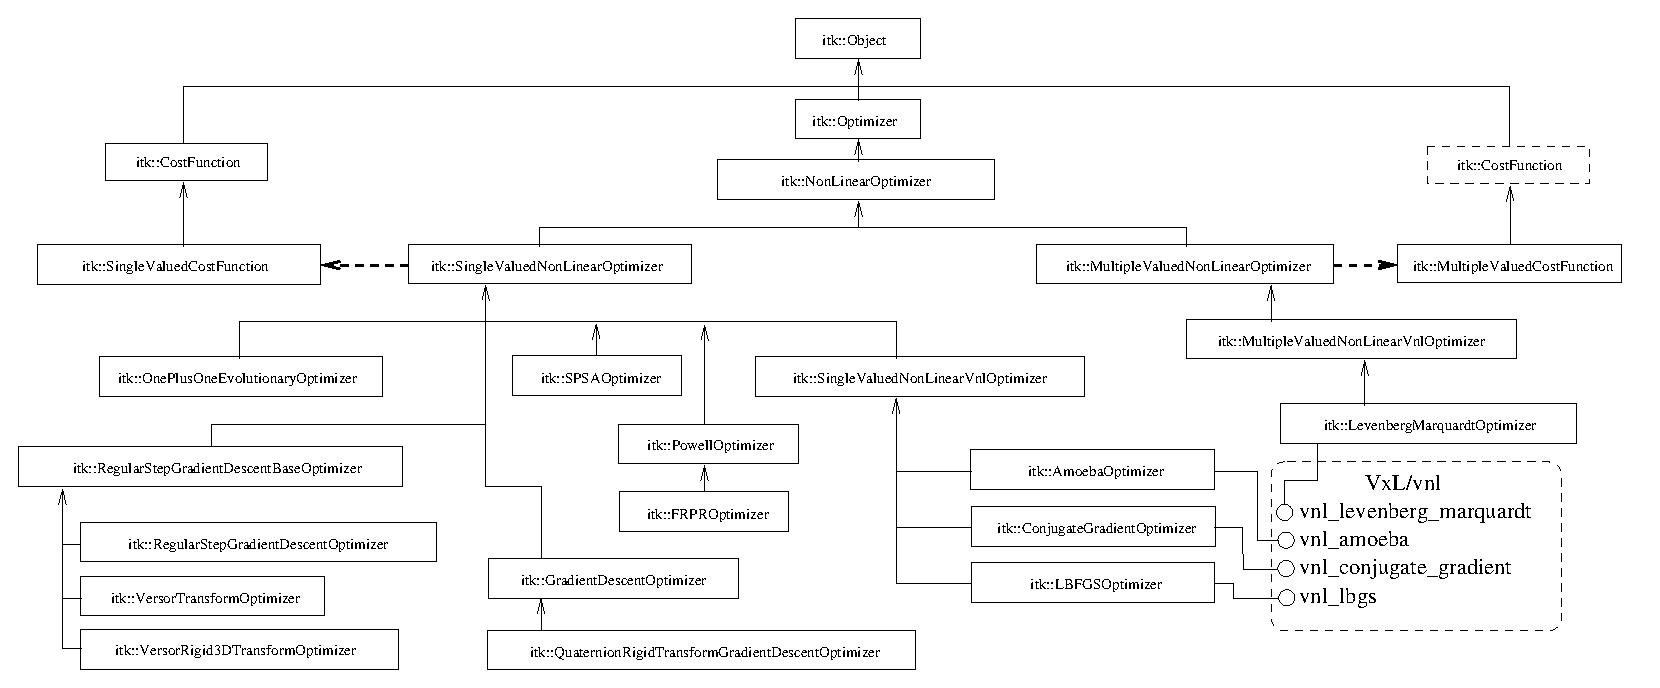
\includegraphics[width=16cm]{OptimizersHierarchy.eps}
\caption{Class diagram of the Optimizers hierarchy.}
\label{fig:OptimizersHierarchy}
\end{figure}

Optimization algorithms are encapsulated as \code{itk::Optimizer} objects
within ITK. Optimizers are generic and can be used for applications other than
registration.  Within the registration framework,
\code{itk::SingleValuedNonLinearOptimizer} are used to optimize the metric
criterion with respect to the transform parameters.

\index{itk::Optimizer!SetInitialPosition()}
\index{itk::Optimizer!StartOptimization()}
\index{itk::Optimizer!GetCurrentPosition()}

The basic input to an optimizer is a cost function object. In the context
of registration, \code{itk::ImageToImageMetric} provide this functionality.
The initial parameters are set using \code{SetInitialPosition()} and
the optimization algorithm is invoked by \code{StartOptimization()}.
Once the optimization has finished, the final parameters can be obtained
using \code{GetCurrentPosition()}.

\index{itk::Optimizer!SetScales()}
Some optimizers also allows rescaling of the individual parameters. This
is convenient for normalizing parameters spaces in which some parameters
have different dynamic ranges. For example, the first parameter of
\code{Euler2DTransform} represent an angle while the last two parameters
the translation. A unit change in angle has a much greater impact on
an image than a unit change in translation. This difference in scale appears
as long narrow valleys in the search space making the optimization problem
diffcult. Rescaling the translation parameters can help to fix this problem.
Scales are represented as \code{Array} of doubles and set defined using
\code{SetScales()}.

The types of \code{itk::SingleValuedNonLinearOptimizer} currently available
in ITK are:

\index{itk::AmoebOptimizer|textbf}
\index{itk::ConjugateGradientOptimizer|textbf}
\index{itk::GradientDescentOptimizer|textbf}
\index{itk::QuaternionRigidTransformGradientDescentOptimizer|textbf}
\index{itk::LBFGSOptimizer|textbf}
\index{itk::OnePlusOneEvolutionaryOptimizer|textbf}
\index{itk::RegularStepGradientDescentOptimizer|textbf}
\index{itk::VersorTransformOptimizer|textbf}
\index{itk::LevenbergMarquardtOptimizer|textbf}

\begin{itemize}

\item \textbf{Amoeba}: Nelder-Meade downhill simplex.  This optimizer is
actually implemented in the \code{VxL/vnl} numerics toolkit.  The ITK class
\code{itk::AmoebaOptimizer} is merely an adaptor class.

\item \textbf{Conjugate Gradient}: Fletcher-Reeves form 
of conjugate gradient with or without preconditioning. Also an adaptor to an
optimizer in \code{vnl}.

\item \textbf{Gradient Descent}: Advance parameters in the direction of the
gradient where the step size is governed by a learning rate. 

\item \textbf{Quaternion Rigid Transform Gradient Descent}: 
A specialized version of \code{GradientDescentOptimizer} for
\code{QuaternionRigidTransform} parameters, where the parameters representing
the quaternion is normalize to a magnitude to one at each iteration to
represent a pure rotation.

\item \textbf{LBFGS}: Limited memory Broyden, Fletcher, Goldfarb
and Shannon minmization. It is an adaptor to an optimizer in \code{vnl}.

\item \textbf{One Plus One Evolutionary}: Strategy that simulates the
biological evolution of a set of samples in the search space. This optimizer
is mainly used in the process of bias correction for MRI images.

\item \textbf{Regular Step Gradient Descent}: Advance parameters in the
direction of the gradient where a bipartition scheme is used to compute
the step size. 

\item \textbf{Versor Transform Optimizer}: A specialized version of
\code{RegularStepGradientDescentOptimizer} for \code{VersorTransform}
parameters  where the current rotation is composed with the gradient rotation
to produce the new rotation vector. It follows the definition of versor
gradients defined by Hamilton~\cite{Hamilton1866}.

\end{itemize}

A parallel hierarchy exists for optimizing multiple-valued cost functions. The
base optimizer in this branch of the hierarchy is the
\code{itk::MultipleValuedNonLinearOptimizer} whose only current derived class
is:

\begin{itemize}

\item \textbf{Levenberg Marquardt}: Non-linear least squares minimization.
Adapted to an optimizer in \code{vnl}.

\end{itemize}


Figure \ref{fig:OptimizersHierarchy} illustrates the full class hierarchy of
optimizers in ITK. Optimizers in the lower right corner are adaptors classes to
optimizers existing in the \code{VxL/vnl} numerics toolkit. The optimizers
interact with the \code{itk::CostFunction} class. In the registration framework
this cost function is reimplemented in the form of \code{itk::ImageToImageMetric}.





